\setcounter{chapter}{2}
\chapter{Research methodology}
\label{chap:3}
\section{Introduction}
The observational and  theoretical understanding of  prompt and  afterglow  phases  of gamma-ray  bursts  suddenly  changed after  20 , November 2004 , the launch of swift equipped with the sophisticated detecting  instruments. Furthermore, the debating  issues  on origins of GRBs ( galactic or cosmological location ) and  the  ( isotropic  or  anisotropic  distributions )  of  GRBs at early  discovery of GRBs  were  confirmed  in  swift era. \\\
Fire ball as  the standard  model   developed  during the  swift era  to  explain  the  emission  mechanisms  of  gamma-ray burst and its  afterglows ( from X-ray to radio  band ). However , the features  of temporal  and  spectral  indices  x-ray afterglow  were not yet clear  as  far  as   review  of  related  literature  concerned . So to solve  this  problem   comprehensive  methodology of  qualitative  and  quantitative research  approach  and  procedures  are  implemented  to  fill the  knowledge  gaps  and  to  explain  unclear  issues  mentioned  in section 1.5 as well.   
\section{Research designs}
\subsection{Fire ball Models}
As  mentioned  in  section (2.2), the  standard   fireball model  proposed   to  explain afterglow   gamma-ray   bursts. In   standard    fireball  model, the   behavior of   X-ray   light curves   assumed  to  be  characterize d   by   a single power   law  and   broken   power   law   decay    model    where flux   fading  time  defined   by : 
\begin{equation}
f_{\nu}(t)\propto  t^{-\alpha} 
\end{equation}
where  $f_{\nu} $the flux decay with time and  $ \alpha  $ is the temporal index/decay slope and subscript by numbers  $ \alpha $ = 1, 2, 3,and 4 for early steep decay slope, shallow or plateau  decay  slope, normal  decay  slope and late  steep  decay slope respectively , that were captured by the swift/XRT. This  is the model that relates both temporal ($ \alpha $) and spectral ( $ \beta $ ) indices  in standard fireball model as:
\begin{equation}
 \alpha  = 2 +   \beta   
\end{equation} is  called the closure relation , where   both  $\beta $  and  $ \alpha $  have  no  units.\\
 \subsection{ spectral  models}
 Several  spectral  functions  models   are   available  for  use  with  gtlike.The  power-law  model  is  the  simplest  model   that   can  be  used   to   describe  a GRB spectrum . This   model   consists   of   two   parameters: the   low-energy   photon index $ \alpha $   and     normalization A.  With   these   two   parameters, the power-law   model   can   fit   the   spectra   of   most   GRBs if   they   are applicable   to   such   a burst.  This   model  is   suitable   when   the  signal-to-noise   ratio   of  the   fitting   spectrum   is   very   low   and  in   the case    when   the   signal  is   weak   and   if   the   break   energy   cannot  be determined   due   to   the    break   energy   of   the   broken  power-law   spectrum   lying   outside   the    energy   band   of   such   a detector. The power-law   spectral   model   for   point   source   is   defined   by   the equation below:[10]
\subsection{ Power law (PL) } 
\begin{equation}
\frac{dN}{dE} = N_{o} (E/ E_{o})^{-\gamma}
\end{equation}
where the parameters in the XML definition have the following mappings:\\
Prefactor = $N_{o}$\\
Index = $\gamma$\\
Scale =$E_{o}$\\
and the units are $ cm^{-2} $ $s^{-2}$ $ MeV^{-2} $. 
\subsection{Numerical models: R-squared  ($ R^{2} $) , covariance and correlation coefficients}
\textbf{ $ R^{2}$ } - R-squared - is the "percent  of variance explained " by  the model. In the  same  token,  it  is   the fraction  by which the variance  of the  error is less than variance. The  values  of   $ R^{2} $  ranges  from  0 to 1  and  typically  expressed  in  percentage , and  defined by  the  equation :
\begin{equation}
R^{2}= \frac{SSR}{ SST}= \frac{\sum (\hat{y_{i}}-\bar{y})^{2}}{\sum(y_{i} -\bar{y})^{2}}
\end{equation}
where SSR- is the sum of square regression or the sum of square residuals.\\
SST -is the total sum square /sum square total.\\
$ \hat{y} $ -is the prediction  or points on the fitting  line.\\
$ \bar{y} $-mean  of all the  values.\\
$ y_{i} $- is  the actual  values / points.\\
  R- squared  also defined as,
 \begin{equation}
 R^{2}= 1- \frac{\sum (\hat{y_{i}}-y_{i})^{2}}{\sum(y_{i} -\bar{y_{i}})^{2}}
\end{equation}   
 The  characteristic  of light  curves  of  gamma-ray afterglows  determined   by   dispersion  of   variables ( numbers of  bursts  versus  time  in  space ).How  far  the   data   spread   or  distributed   around  the  mean / average   values  explained   by   correlation  and  covariance . The  covariance  of two dimensional  data defined as :
\begin{equation}
cov(x,y) = \frac{1}{n-1}\sum_{i=1}^{n}{(x_{i}- \bar{x} )}{(y_{i}-\bar{y} )}
\end{equation}   
Similarly ,  correlation  coefficient  of the same  data given by :  	 
\begin{equation}
r_{xy} = \frac{1}{n-1}\sum_{i=1}^{n}\frac{(x_{i}- \bar{x}  )}{sd(x)}\frac{(y_{i}-  \bar{y} )}{sd(y)}
\end{equation}
If   covaiance  C ( x, y ) of two dimensional  data  were  known , we  use the equation:
\begin{equation}
r_{xy} = \frac{cov(xy)}{\sqrt{v(x)v(y)}}
\end{equation},
where  cov ( x , y )  is   covariance ,  sd(x)  and  sd(y)  are  standard  divaition  of   x-data  and  y-data  and  they  are square root  of  variance  v( x ) and  v(y)  respectively .The  values  of  covariance  of the  data  lies   in  the  range  of   $-\infty$  and  $+\infty$ ,   where  as   the   values   of  correlation   coefficient  $ r_{xy} $  limited     b/n   range  -1.00   and  +1.00 . The  results  of  data analysis :  C ( x, y)  and  $ r_{xy} $  presented  in  table     $r_{xy}$  is  correlation   coefficient  of   x-data   and   y-data . In   our  case, x-data  and y-data  represent  time (sec)  and  flux  in  $(erg /cm^{-2} s^{-1}) $ respectively .	
\section{Type of data  and its source }
For  our  work , we  used   the   existing  secondary   data  type  detected by  Swift-XRT   ( evans et.al   Online  repository )  over  longer  periods. In our sample , both  the   classes   of  gamma-ray   bursts  (short  and  long  GRBs )  are  selected equally. 
\section{Data sampling technique and size}
Three   Criterion  were  designed   to   select   the  required   sample. i.e  types of  gamma-ray   , the   number  of   light  curve   breaks   and  well  defined  red shifts   are   used   to   select   the   desired   sampled  data.  Based  on mentioned   criterion ,  twenty  (20)  GRBs   afterglows   are   selected   using  simple   random   probability   sampling   method. The   sampled   GRBs   afterglow  data   tabulated in table  below.
\begin{center}
\begin{table}
\caption{\label{tab:"Table 3.1: " } Represents    swift / xrt  data sampled  for  long and short  grb   }
\begin{tabular}{|l|l|l|l|l|} 
\hline
Class of GRBs & LC with Break 1 & LC with Break 2 & LC with Break 3 & Total \\ \hline
Short GRB & 2 & 3 & 5 & 10 \\ \hline
Long GRB & 3 & 2 & 5 & 10 \\ \hline
Total & 5 & 5 & 10 & 20 \\ \hline 
\end{tabular}
\end{table}
\end{center}
\section{Validity and reliability of data }
 As mentioned in section 3.3, examine the data then to get the information about object under taken , we already decided to follow both quantitative and qualitative approaches , standard models and tools were  proposed  to use in analyzing the data collected so as to achieve the desired  objectives and  answers  for the  statements of problems mentioned in section 1.5. This might be  keep the validity and reliability of our work.
\section{Data processing and analyzing} 
\subsection{Data processing }
As mentioned in section 3.3 above ,  twenty  gamma -ray bursts ( long and short ) were  collected   as  a sample to  analyze. To extract relevant information and conclusions  that support   the  final  judgment ,  the sampled  GRBs  data   were cleaned by avoiding  duplicated  , incorrect  ,  and  missing  data .  
\subsection{Data analyzing}
We  analyze    our  sampled  swift / xrt  data  to   calculate  the  fitting  parameters ( temporal indices  ,   amplitudes and  covariance   etc ) , furthermore  to   observe   and  test  how  these   parameters   determine  the  features of  light curves  of  x-ray afterglows .  using   power law model  and  applying  python 3  programming   language ,  the  plot  of  flux (F)  against  time (t)  of  sampled  x-ray  data has been shown  respectively  for long and short  GRBs in fig......and....fig  below .  The  results  of Calculated   fitting  parameters   are  also  tabulated in  table (a) and (b) section 4.1.
\begin{figure}[hpbt]
\subfloat[] {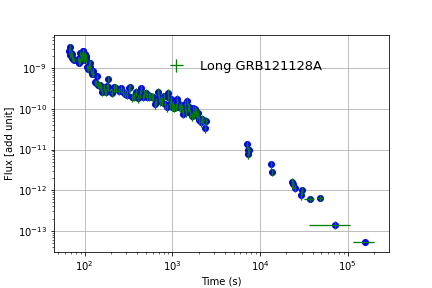
\includegraphics[scale=0.4]{Figures/121128A_err.png}}
\subfloat[] {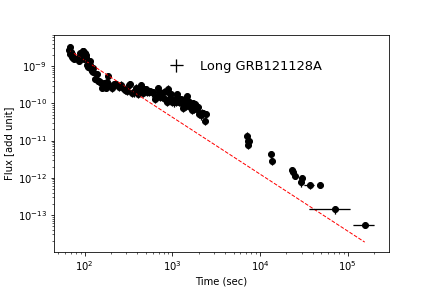
\includegraphics[scale=0.4]{Figures/121128A_fit.png}}
\subfloat[] {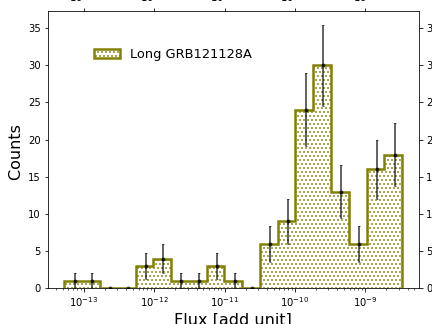
\includegraphics[scale=0.3]{Figures/121128A_hist.png}}
\caption{x-ray  afterglow Light curve (a) , x-ray  light curve fitting - red line (b) , and histogram  of  photons counts  versus x-ray flux  (c)  of long GRB121128A .}
\end{figure}
\begin{figure}[hpbt]
\subfloat[] {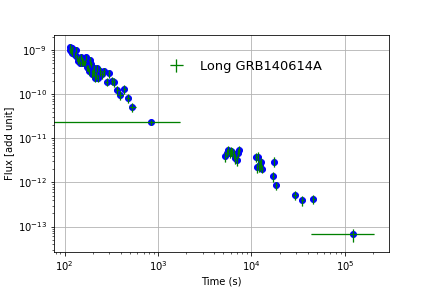
\includegraphics[scale=0.4]{Figures/140614A_err.png}}
\subfloat[] {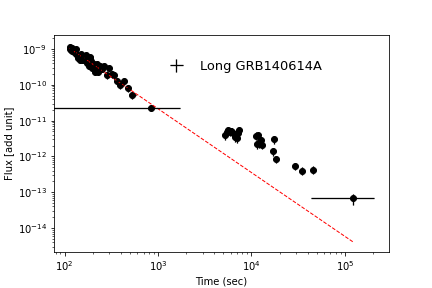
\includegraphics[scale=0.4]{Figures/140614A_fit.png}}
\subfloat[] {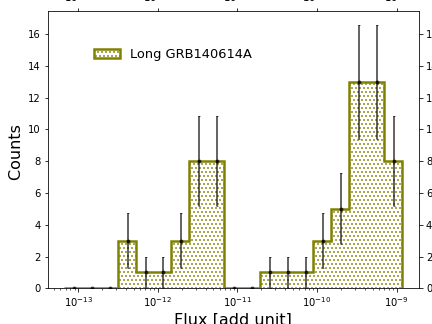
\includegraphics[scale=0.3]{Figures/140614A_hist.png}}
\caption{x-ray  afterglow Light curve (a) , x-ray  light curve fitting - red line (b) , and histogram  of  photons counts  versus x-ray flux  (c)  of long GRB140614A .}
\end{figure}
\begin{figure}[hpbt]
\subfloat[] {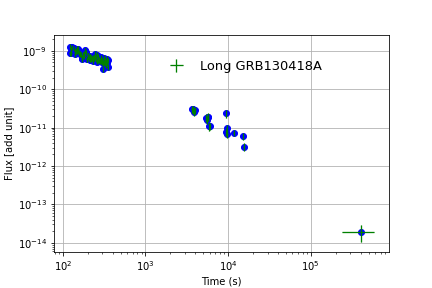
\includegraphics[scale=0.4]{Figures/130418A_err.png}}
\subfloat[] {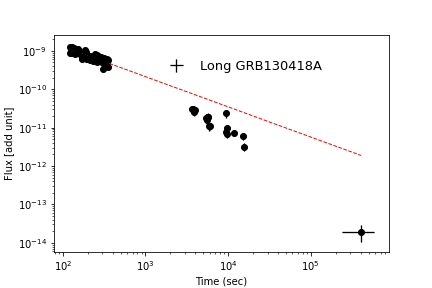
\includegraphics[scale=0.4]{Figures/130418A_fit.png}}
\subfloat[] {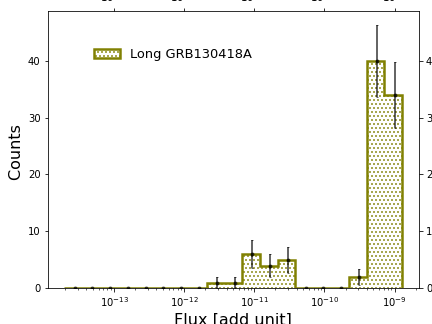
\includegraphics[scale=0.3]{Figures/130418A_hist.png}}
\caption{x-ray  afterglow Light curve (a) , x-ray  light curve fitting - red line (b) , and histogram  of  photons counts  versus x-ray flux  (c)  of long GRB130418A .}
\end{figure}
\begin{figure}[hpbt]
\subfloat[] {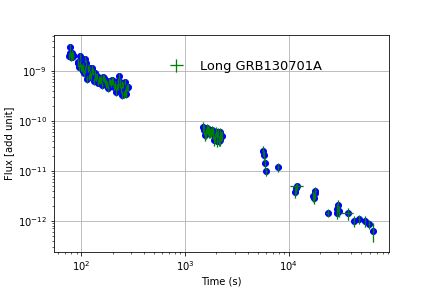
\includegraphics[scale=0.4]{Figures/130701A_err.png}}
\subfloat[] {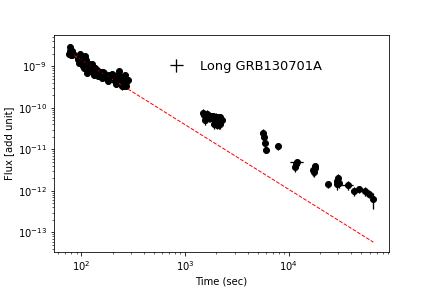
\includegraphics[scale=0.4]{Figures/130701A_fit.png}}
\subfloat[] {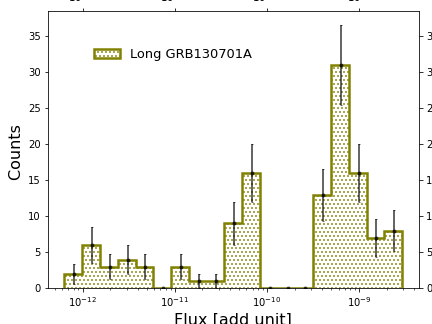
\includegraphics[scale=0.3]{Figures/130701A_hist.png}}
\caption{x-ray  afterglow Light curve (a) , x-ray  light curve fitting - red line (b) , and histogram  of  photons counts  versus x-ray flux  (c)  of long GRB130701A .}
\end{figure}
\begin{figure}[hpbt]
\subfloat[] {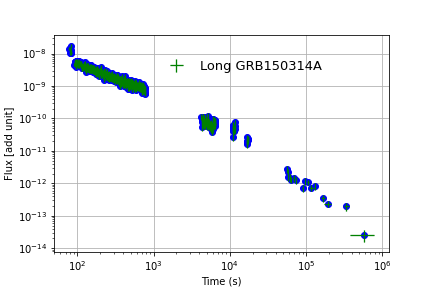
\includegraphics[scale=0.4]{Figures/150314A_err.png}}
\subfloat[] {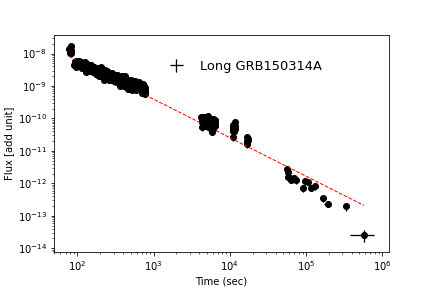
\includegraphics[scale=0.4]{Figures/150314A_fit.png}}
\subfloat[] {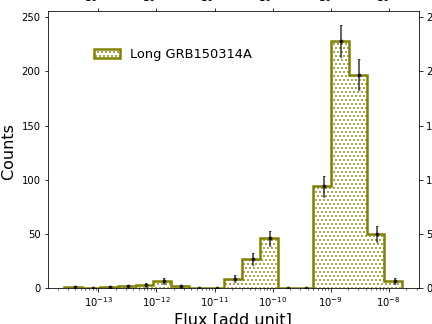
\includegraphics[scale=0.3]{Figures/150314A_hist.png}}
\caption{x-ray  afterglow Light curve (a) , x-ray  light curve fitting - red line (b) , and histogram  of  photons counts  versus x-ray flux  (c)  of long GRB150314A .}
\end{figure}
using python 3 programming language the fitting of five short GRBs have been performed and shown in figures below.
\begin{figure}[hpbt]
\subfloat[] {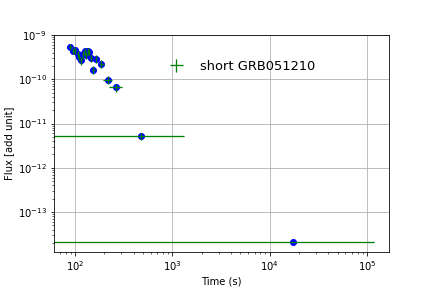
\includegraphics[scale=0.4]{Figures/051210_err.png}}
\subfloat[] {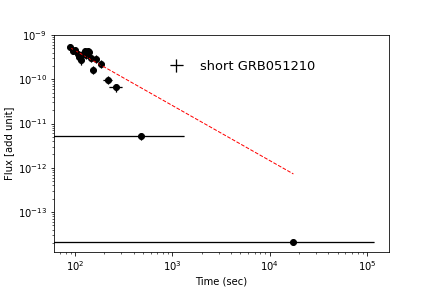
\includegraphics[scale=0.4]{Figures/051210_fit.png}}
\subfloat[] {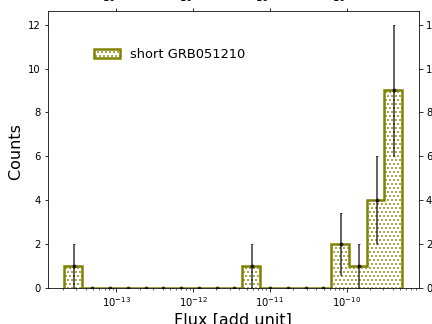
\includegraphics[scale=0.3]{Figures/051210_hist.png}}
\caption{x-ray  afterglow Light curve (a) , x-ray  light curve fitting - red line (b) , and histogram  of  photons counts  versus x-ray flux  (c)  of short GRB051210 .}
\end{figure}
\begin{figure}[hpbt]
\subfloat[] {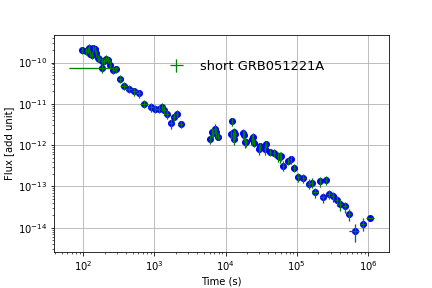
\includegraphics[scale=0.4]{Figures/051221A_err.png}}
\subfloat[] {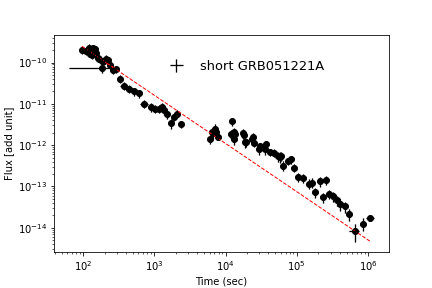
\includegraphics[scale=0.4]{Figures/051221A_fit.png}}
\subfloat[] {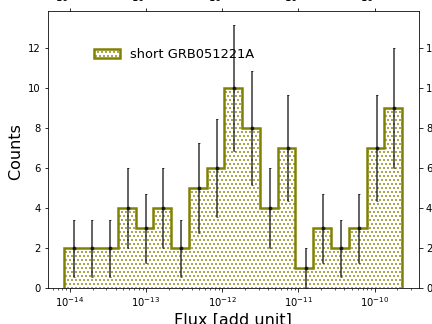
\includegraphics[scale=0.3]{Figures/051221A_hist.png}}
\caption{x-ray  afterglow Light curve (a) , x-ray  light curve fitting - red line (b) , and histogram  of  photons counts  versus x-ray flux  (c)  of short GRB 051221A.}
\end{figure}
\begin{figure}[hpbt]
\subfloat[] {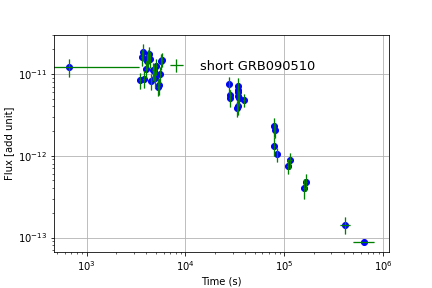
\includegraphics[scale=0.4]{Figures/090510_err.png}}
\subfloat[] {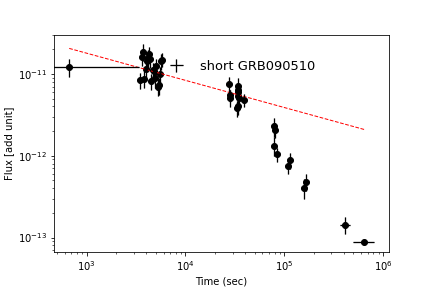
\includegraphics[scale=0.4]{Figures/090510_fit.png}}
\subfloat[] {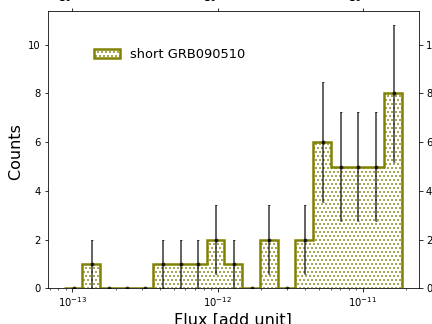
\includegraphics[scale=0.3]{Figures/090510_hist.png}}
\caption{x-ray  afterglow Light curve (a) , x-ray  light curve fitting - red line (b) , and histogram  of  photons counts  versus x-ray flux  (c)  of short GRB090510.}
\end{figure}
\begin{figure}[hpbt]
\subfloat[]{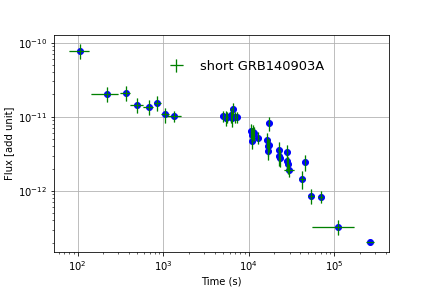
\includegraphics[scale=0.4]{Figures/140903A_err.png}}
\subfloat[]{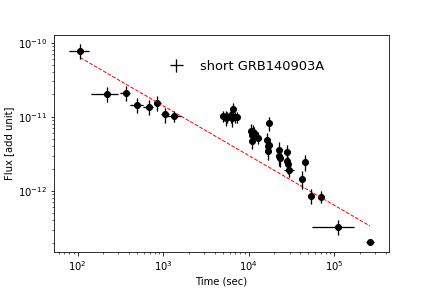
\includegraphics[scale=0.4]{Figures/140903A_fit.png}}
\subfloat[]{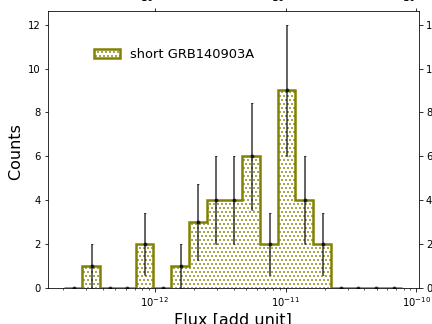
\includegraphics[scale=0.3]{Figures/140903A_hist.png}}
\caption{x-ray  afterglow Light curve (a) , x-ray  light curve fitting - red line (b) , and histogram  of  photons counts  versus x-ray flux  (c)  of short GRB140903A.}
\end{figure}  
\begin{figure}[hpbt]
\subfloat[]{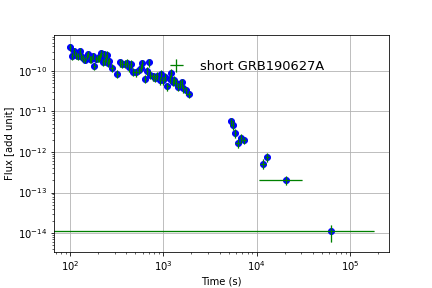
\includegraphics[scale=0.4]{Figures/190627A_err.png}}
\subfloat[]{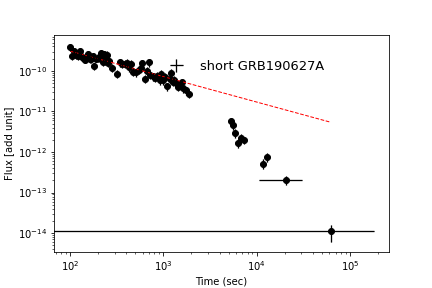
\includegraphics[scale=0.4]{Figures/190627A_fit.png}}
\subfloat[]{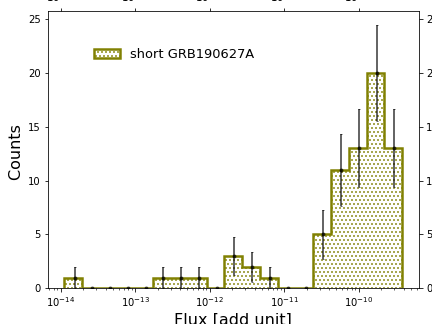
\includegraphics[scale=0.3]{Figures/190627A_hist.png}}
\caption{x-ray  afterglow Light curve (a) , x-ray  light curve fitting - red line (b) , and histogram  of  photons counts  versus x-ray flux  (c)  of short GRB190627A.}
\end{figure}\\\\
